%% fig_hodgecount.tex   (generated by make_frontier.py; do not edit by hand)
%% Hodge classes of the square of a Mumford fourfold, degree by degree, against the subring generated by divisor classes.
\documentclass[tikz,border=6pt]{standalone}
\usepackage{amsmath,amssymb}
\usetikzlibrary{arrows.meta,calc,decorations.pathreplacing,patterns}
%% palette.tex -- shared colour definitions for the figures
\definecolor{PInk}{RGB}{26,32,44}
\definecolor{PBlue}{RGB}{37,82,139}
\definecolor{PTeal}{RGB}{23,127,125}
\definecolor{POchre}{RGB}{193,138,44}
\definecolor{PClay}{RGB}{178,74,58}
\definecolor{PSlate}{RGB}{108,122,137}
\definecolor{PViolet}{RGB}{110,86,150}
\definecolor{WBlue}{RGB}{223,234,246}
\definecolor{WTeal}{RGB}{220,238,236}
\definecolor{WOchre}{RGB}{250,240,218}
\definecolor{WClay}{RGB}{247,229,224}
\definecolor{WSlate}{RGB}{238,241,244}
\definecolor{PMag}{RGB}{158,58,110}
\definecolor{PGrass}{RGB}{62,124,66}
\definecolor{PAmber}{RGB}{214,112,38}
\definecolor{PIndigo}{RGB}{58,64,140}
\definecolor{PRule}{RGB}{176,186,197}

%% shared macros so the standalone figures match the paper
\providecommand{\QQ}{\mathbb{Q}}
\providecommand{\ZZ}{\mathbb{Z}}
\providecommand{\RR}{\mathbb{R}}
\providecommand{\CC}{\mathbb{C}}
\providecommand{\PP}{\mathbb{P}}
\providecommand{\Kx}{K^{\times}}
\providecommand{\HW}{W}
\providecommand{\Nm}{\mathrm{N}}
\providecommand{\Hdg}{\mathrm{Hdg}}
\providecommand{\NS}{\mathrm{NS}}
\providecommand{\cA}{\mathcal{A}}
\providecommand{\cD}{\mathcal{D}}
\providecommand{\cF}{\mathcal{F}}
\providecommand{\cP}{\mathcal{P}}
\providecommand{\cO}{\mathcal{O}}
\providecommand{\cQ}{\mathcal{Q}}
\providecommand{\bbar}[1]{\overline{#1}}
\providecommand{\ch}{\operatorname{ch}}
\providecommand{\End}{\mathrm{End}}
\providecommand{\Ext}{\operatorname{Ext}}
\providecommand{\Supp}{\operatorname{Supp}}

\begin{document}
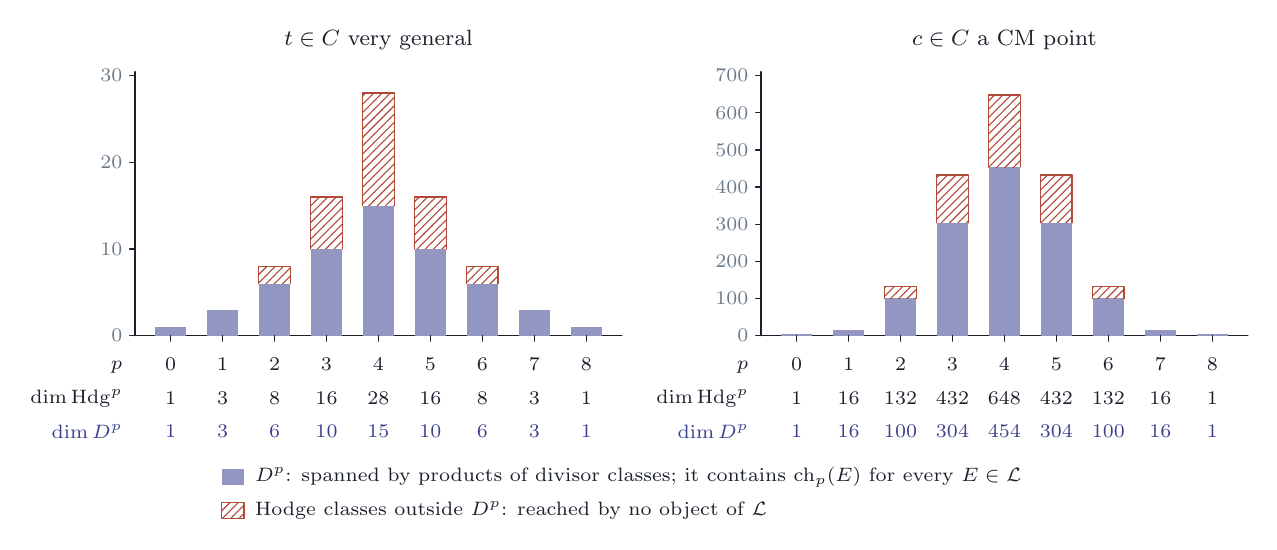
\begin{tikzpicture}[x=1cm,y=1cm,line join=round,line cap=round,
  font=\small,text=PInk]
  \draw[PInk,line width=0.60pt] (0.100,0.000) -- (6.280,0.000);
  \draw[PInk,line width=0.60pt] (0.100,0.000) -- (0.100,3.350);
  \draw[PInk,line width=0.50pt] (0.030,0.000) -- (0.100,0.000);
  \node[text=PSlate,inner sep=1pt,align=center,font=\scriptsize,anchor=east] at (-0.020,0.000) {$0$};
  \draw[PInk,line width=0.50pt] (0.030,1.100) -- (0.100,1.100);
  \node[text=PSlate,inner sep=1pt,align=center,font=\scriptsize,anchor=east] at (-0.020,1.100) {$10$};
  \draw[PInk,line width=0.50pt] (0.030,2.200) -- (0.100,2.200);
  \node[text=PSlate,inner sep=1pt,align=center,font=\scriptsize,anchor=east] at (-0.020,2.200) {$20$};
  \draw[PInk,line width=0.50pt] (0.030,3.300) -- (0.100,3.300);
  \node[text=PSlate,inner sep=1pt,align=center,font=\scriptsize,anchor=east] at (-0.020,3.300) {$30$};
  \fill[PIndigo!55] (0.350,0.000) -- (0.750,0.000) -- (0.750,0.110) -- (0.350,0.110) -- cycle;
  \draw[PInk,line width=0.50pt] (0.550,0.000) -- (0.550,-0.070);
  \node[text=PInk,inner sep=1pt,align=center,font=\scriptsize] at (0.550,-0.360) {$0$};
  \node[text=PInk,inner sep=1pt,align=center,font=\scriptsize] at (0.550,-0.800) {$1$};
  \node[text=PIndigo,inner sep=1pt,align=center,font=\scriptsize] at (0.550,-1.220) {$1$};
  \fill[PIndigo!55] (1.010,0.000) -- (1.410,0.000) -- (1.410,0.330) -- (1.010,0.330) -- cycle;
  \draw[PInk,line width=0.50pt] (1.210,0.000) -- (1.210,-0.070);
  \node[text=PInk,inner sep=1pt,align=center,font=\scriptsize] at (1.210,-0.360) {$1$};
  \node[text=PInk,inner sep=1pt,align=center,font=\scriptsize] at (1.210,-0.800) {$3$};
  \node[text=PIndigo,inner sep=1pt,align=center,font=\scriptsize] at (1.210,-1.220) {$3$};
  \fill[PIndigo!55] (1.670,0.000) -- (2.070,0.000) -- (2.070,0.660) -- (1.670,0.660) -- cycle;
  \fill[pattern=north east lines,pattern color=PClay] (1.670,0.660) rectangle (2.070,0.880);
  \draw[PClay,line width=0.50pt] (1.670,0.660) -- (1.670,0.880) -- (2.070,0.880) -- (2.070,0.660);
  \draw[PInk,line width=0.50pt] (1.870,0.000) -- (1.870,-0.070);
  \node[text=PInk,inner sep=1pt,align=center,font=\scriptsize] at (1.870,-0.360) {$2$};
  \node[text=PInk,inner sep=1pt,align=center,font=\scriptsize] at (1.870,-0.800) {$8$};
  \node[text=PIndigo,inner sep=1pt,align=center,font=\scriptsize] at (1.870,-1.220) {$6$};
  \fill[PIndigo!55] (2.330,0.000) -- (2.730,0.000) -- (2.730,1.100) -- (2.330,1.100) -- cycle;
  \fill[pattern=north east lines,pattern color=PClay] (2.330,1.100) rectangle (2.730,1.760);
  \draw[PClay,line width=0.50pt] (2.330,1.100) -- (2.330,1.760) -- (2.730,1.760) -- (2.730,1.100);
  \draw[PInk,line width=0.50pt] (2.530,0.000) -- (2.530,-0.070);
  \node[text=PInk,inner sep=1pt,align=center,font=\scriptsize] at (2.530,-0.360) {$3$};
  \node[text=PInk,inner sep=1pt,align=center,font=\scriptsize] at (2.530,-0.800) {$16$};
  \node[text=PIndigo,inner sep=1pt,align=center,font=\scriptsize] at (2.530,-1.220) {$10$};
  \fill[PIndigo!55] (2.990,0.000) -- (3.390,0.000) -- (3.390,1.650) -- (2.990,1.650) -- cycle;
  \fill[pattern=north east lines,pattern color=PClay] (2.990,1.650) rectangle (3.390,3.080);
  \draw[PClay,line width=0.50pt] (2.990,1.650) -- (2.990,3.080) -- (3.390,3.080) -- (3.390,1.650);
  \draw[PInk,line width=0.50pt] (3.190,0.000) -- (3.190,-0.070);
  \node[text=PInk,inner sep=1pt,align=center,font=\scriptsize] at (3.190,-0.360) {$4$};
  \node[text=PInk,inner sep=1pt,align=center,font=\scriptsize] at (3.190,-0.800) {$28$};
  \node[text=PIndigo,inner sep=1pt,align=center,font=\scriptsize] at (3.190,-1.220) {$15$};
  \fill[PIndigo!55] (3.650,0.000) -- (4.050,0.000) -- (4.050,1.100) -- (3.650,1.100) -- cycle;
  \fill[pattern=north east lines,pattern color=PClay] (3.650,1.100) rectangle (4.050,1.760);
  \draw[PClay,line width=0.50pt] (3.650,1.100) -- (3.650,1.760) -- (4.050,1.760) -- (4.050,1.100);
  \draw[PInk,line width=0.50pt] (3.850,0.000) -- (3.850,-0.070);
  \node[text=PInk,inner sep=1pt,align=center,font=\scriptsize] at (3.850,-0.360) {$5$};
  \node[text=PInk,inner sep=1pt,align=center,font=\scriptsize] at (3.850,-0.800) {$16$};
  \node[text=PIndigo,inner sep=1pt,align=center,font=\scriptsize] at (3.850,-1.220) {$10$};
  \fill[PIndigo!55] (4.310,0.000) -- (4.710,0.000) -- (4.710,0.660) -- (4.310,0.660) -- cycle;
  \fill[pattern=north east lines,pattern color=PClay] (4.310,0.660) rectangle (4.710,0.880);
  \draw[PClay,line width=0.50pt] (4.310,0.660) -- (4.310,0.880) -- (4.710,0.880) -- (4.710,0.660);
  \draw[PInk,line width=0.50pt] (4.510,0.000) -- (4.510,-0.070);
  \node[text=PInk,inner sep=1pt,align=center,font=\scriptsize] at (4.510,-0.360) {$6$};
  \node[text=PInk,inner sep=1pt,align=center,font=\scriptsize] at (4.510,-0.800) {$8$};
  \node[text=PIndigo,inner sep=1pt,align=center,font=\scriptsize] at (4.510,-1.220) {$6$};
  \fill[PIndigo!55] (4.970,0.000) -- (5.370,0.000) -- (5.370,0.330) -- (4.970,0.330) -- cycle;
  \draw[PInk,line width=0.50pt] (5.170,0.000) -- (5.170,-0.070);
  \node[text=PInk,inner sep=1pt,align=center,font=\scriptsize] at (5.170,-0.360) {$7$};
  \node[text=PInk,inner sep=1pt,align=center,font=\scriptsize] at (5.170,-0.800) {$3$};
  \node[text=PIndigo,inner sep=1pt,align=center,font=\scriptsize] at (5.170,-1.220) {$3$};
  \fill[PIndigo!55] (5.630,0.000) -- (6.030,0.000) -- (6.030,0.110) -- (5.630,0.110) -- cycle;
  \draw[PInk,line width=0.50pt] (5.830,0.000) -- (5.830,-0.070);
  \node[text=PInk,inner sep=1pt,align=center,font=\scriptsize] at (5.830,-0.360) {$8$};
  \node[text=PInk,inner sep=1pt,align=center,font=\scriptsize] at (5.830,-0.800) {$1$};
  \node[text=PIndigo,inner sep=1pt,align=center,font=\scriptsize] at (5.830,-1.220) {$1$};
  \node[text=PInk,inner sep=1pt,align=center,font=\scriptsize,anchor=east] at (-0.020,-0.800) {$\dim\mathrm{Hdg}^{p}$};
  \node[text=PIndigo,inner sep=1pt,align=center,font=\scriptsize,anchor=east] at (-0.020,-1.220) {$\dim D^{p}$};
  \node[text=PInk,inner sep=1pt,align=center,font=\scriptsize,anchor=east] at (-0.020,-0.400) {$p$};
  \node[text=PInk,inner sep=1pt,align=center,font=\footnotesize] at (3.190,3.750) {$t\in C$ very general};
  \draw[PInk,line width=0.60pt] (8.050,0.000) -- (14.230,0.000);
  \draw[PInk,line width=0.60pt] (8.050,0.000) -- (8.050,3.350);
  \draw[PInk,line width=0.50pt] (7.980,0.000) -- (8.050,0.000);
  \node[text=PSlate,inner sep=1pt,align=center,font=\scriptsize,anchor=east] at (7.930,0.000) {$0$};
  \draw[PInk,line width=0.50pt] (7.980,0.471) -- (8.050,0.471);
  \node[text=PSlate,inner sep=1pt,align=center,font=\scriptsize,anchor=east] at (7.930,0.471) {$100$};
  \draw[PInk,line width=0.50pt] (7.980,0.943) -- (8.050,0.943);
  \node[text=PSlate,inner sep=1pt,align=center,font=\scriptsize,anchor=east] at (7.930,0.943) {$200$};
  \draw[PInk,line width=0.50pt] (7.980,1.414) -- (8.050,1.414);
  \node[text=PSlate,inner sep=1pt,align=center,font=\scriptsize,anchor=east] at (7.930,1.414) {$300$};
  \draw[PInk,line width=0.50pt] (7.980,1.886) -- (8.050,1.886);
  \node[text=PSlate,inner sep=1pt,align=center,font=\scriptsize,anchor=east] at (7.930,1.886) {$400$};
  \draw[PInk,line width=0.50pt] (7.980,2.357) -- (8.050,2.357);
  \node[text=PSlate,inner sep=1pt,align=center,font=\scriptsize,anchor=east] at (7.930,2.357) {$500$};
  \draw[PInk,line width=0.50pt] (7.980,2.829) -- (8.050,2.829);
  \node[text=PSlate,inner sep=1pt,align=center,font=\scriptsize,anchor=east] at (7.930,2.829) {$600$};
  \draw[PInk,line width=0.50pt] (7.980,3.300) -- (8.050,3.300);
  \node[text=PSlate,inner sep=1pt,align=center,font=\scriptsize,anchor=east] at (7.930,3.300) {$700$};
  \fill[PIndigo!55] (8.300,0.000) -- (8.700,0.000) -- (8.700,0.020) -- (8.300,0.020) -- cycle;
  \draw[PInk,line width=0.50pt] (8.500,0.000) -- (8.500,-0.070);
  \node[text=PInk,inner sep=1pt,align=center,font=\scriptsize] at (8.500,-0.360) {$0$};
  \node[text=PInk,inner sep=1pt,align=center,font=\scriptsize] at (8.500,-0.800) {$1$};
  \node[text=PIndigo,inner sep=1pt,align=center,font=\scriptsize] at (8.500,-1.220) {$1$};
  \fill[PIndigo!55] (8.960,0.000) -- (9.360,0.000) -- (9.360,0.075) -- (8.960,0.075) -- cycle;
  \draw[PInk,line width=0.50pt] (9.160,0.000) -- (9.160,-0.070);
  \node[text=PInk,inner sep=1pt,align=center,font=\scriptsize] at (9.160,-0.360) {$1$};
  \node[text=PInk,inner sep=1pt,align=center,font=\scriptsize] at (9.160,-0.800) {$16$};
  \node[text=PIndigo,inner sep=1pt,align=center,font=\scriptsize] at (9.160,-1.220) {$16$};
  \fill[PIndigo!55] (9.620,0.000) -- (10.020,0.000) -- (10.020,0.471) -- (9.620,0.471) -- cycle;
  \fill[pattern=north east lines,pattern color=PClay] (9.620,0.471) rectangle (10.020,0.622);
  \draw[PClay,line width=0.50pt] (9.620,0.471) -- (9.620,0.622) -- (10.020,0.622) -- (10.020,0.471);
  \draw[PInk,line width=0.50pt] (9.820,0.000) -- (9.820,-0.070);
  \node[text=PInk,inner sep=1pt,align=center,font=\scriptsize] at (9.820,-0.360) {$2$};
  \node[text=PInk,inner sep=1pt,align=center,font=\scriptsize] at (9.820,-0.800) {$132$};
  \node[text=PIndigo,inner sep=1pt,align=center,font=\scriptsize] at (9.820,-1.220) {$100$};
  \fill[PIndigo!55] (10.280,0.000) -- (10.680,0.000) -- (10.680,1.433) -- (10.280,1.433) -- cycle;
  \fill[pattern=north east lines,pattern color=PClay] (10.280,1.433) rectangle (10.680,2.037);
  \draw[PClay,line width=0.50pt] (10.280,1.433) -- (10.280,2.037) -- (10.680,2.037) -- (10.680,1.433);
  \draw[PInk,line width=0.50pt] (10.480,0.000) -- (10.480,-0.070);
  \node[text=PInk,inner sep=1pt,align=center,font=\scriptsize] at (10.480,-0.360) {$3$};
  \node[text=PInk,inner sep=1pt,align=center,font=\scriptsize] at (10.480,-0.800) {$432$};
  \node[text=PIndigo,inner sep=1pt,align=center,font=\scriptsize] at (10.480,-1.220) {$304$};
  \fill[PIndigo!55] (10.940,0.000) -- (11.340,0.000) -- (11.340,2.140) -- (10.940,2.140) -- cycle;
  \fill[pattern=north east lines,pattern color=PClay] (10.940,2.140) rectangle (11.340,3.055);
  \draw[PClay,line width=0.50pt] (10.940,2.140) -- (10.940,3.055) -- (11.340,3.055) -- (11.340,2.140);
  \draw[PInk,line width=0.50pt] (11.140,0.000) -- (11.140,-0.070);
  \node[text=PInk,inner sep=1pt,align=center,font=\scriptsize] at (11.140,-0.360) {$4$};
  \node[text=PInk,inner sep=1pt,align=center,font=\scriptsize] at (11.140,-0.800) {$648$};
  \node[text=PIndigo,inner sep=1pt,align=center,font=\scriptsize] at (11.140,-1.220) {$454$};
  \fill[PIndigo!55] (11.600,0.000) -- (12.000,0.000) -- (12.000,1.433) -- (11.600,1.433) -- cycle;
  \fill[pattern=north east lines,pattern color=PClay] (11.600,1.433) rectangle (12.000,2.037);
  \draw[PClay,line width=0.50pt] (11.600,1.433) -- (11.600,2.037) -- (12.000,2.037) -- (12.000,1.433);
  \draw[PInk,line width=0.50pt] (11.800,0.000) -- (11.800,-0.070);
  \node[text=PInk,inner sep=1pt,align=center,font=\scriptsize] at (11.800,-0.360) {$5$};
  \node[text=PInk,inner sep=1pt,align=center,font=\scriptsize] at (11.800,-0.800) {$432$};
  \node[text=PIndigo,inner sep=1pt,align=center,font=\scriptsize] at (11.800,-1.220) {$304$};
  \fill[PIndigo!55] (12.260,0.000) -- (12.660,0.000) -- (12.660,0.471) -- (12.260,0.471) -- cycle;
  \fill[pattern=north east lines,pattern color=PClay] (12.260,0.471) rectangle (12.660,0.622);
  \draw[PClay,line width=0.50pt] (12.260,0.471) -- (12.260,0.622) -- (12.660,0.622) -- (12.660,0.471);
  \draw[PInk,line width=0.50pt] (12.460,0.000) -- (12.460,-0.070);
  \node[text=PInk,inner sep=1pt,align=center,font=\scriptsize] at (12.460,-0.360) {$6$};
  \node[text=PInk,inner sep=1pt,align=center,font=\scriptsize] at (12.460,-0.800) {$132$};
  \node[text=PIndigo,inner sep=1pt,align=center,font=\scriptsize] at (12.460,-1.220) {$100$};
  \fill[PIndigo!55] (12.920,0.000) -- (13.320,0.000) -- (13.320,0.075) -- (12.920,0.075) -- cycle;
  \draw[PInk,line width=0.50pt] (13.120,0.000) -- (13.120,-0.070);
  \node[text=PInk,inner sep=1pt,align=center,font=\scriptsize] at (13.120,-0.360) {$7$};
  \node[text=PInk,inner sep=1pt,align=center,font=\scriptsize] at (13.120,-0.800) {$16$};
  \node[text=PIndigo,inner sep=1pt,align=center,font=\scriptsize] at (13.120,-1.220) {$16$};
  \fill[PIndigo!55] (13.580,0.000) -- (13.980,0.000) -- (13.980,0.020) -- (13.580,0.020) -- cycle;
  \draw[PInk,line width=0.50pt] (13.780,0.000) -- (13.780,-0.070);
  \node[text=PInk,inner sep=1pt,align=center,font=\scriptsize] at (13.780,-0.360) {$8$};
  \node[text=PInk,inner sep=1pt,align=center,font=\scriptsize] at (13.780,-0.800) {$1$};
  \node[text=PIndigo,inner sep=1pt,align=center,font=\scriptsize] at (13.780,-1.220) {$1$};
  \node[text=PInk,inner sep=1pt,align=center,font=\scriptsize,anchor=east] at (7.930,-0.800) {$\dim\mathrm{Hdg}^{p}$};
  \node[text=PIndigo,inner sep=1pt,align=center,font=\scriptsize,anchor=east] at (7.930,-1.220) {$\dim D^{p}$};
  \node[text=PInk,inner sep=1pt,align=center,font=\scriptsize,anchor=east] at (7.930,-0.400) {$p$};
  \node[text=PInk,inner sep=1pt,align=center,font=\footnotesize] at (11.140,3.750) {$c\in C$ a CM point};
  \fill[PIndigo!55] (1.200,-1.900) -- (1.480,-1.900) -- (1.480,-1.700) -- (1.200,-1.700) -- cycle;
  \node[text=PInk,inner sep=1pt,align=center,font=\scriptsize,anchor=west] at (1.580,-1.800) {$D^{p}$: spanned by products of divisor classes; it contains $\mathrm{ch}_{p}(E)$ for every $E\in\mathcal{L}$};
  \fill[pattern=north east lines,pattern color=PClay] (1.20,-2.320) rectangle (1.48,-2.120);
  \draw[PClay,line width=0.50pt] (1.200,-2.320) -- (1.480,-2.320) -- (1.480,-2.120) -- (1.200,-2.120) -- (1.200,-2.320);
  \node[text=PInk,inner sep=1pt,align=center,font=\scriptsize,anchor=west] at (1.580,-2.220) {Hodge classes outside $D^{p}$: reached by no object of $\mathcal{L}$};
\end{tikzpicture}
\end{document}
